% The agent loop and its tools (phase 3, POST /api/chat).
% Build: tectonic --outdir . fig-agent-v1.tex
\documentclass[border=16pt]{standalone}
\usepackage[T1]{fontenc}
\usepackage[utf8]{inputenc}
\usepackage{helvet}
\renewcommand{\familydefault}{\sfdefault}
\usepackage[none]{hyphenat}
\usepackage{tikz}
\usetikzlibrary{arrows.meta,calc,shapes.geometric}

\definecolor{ink}{HTML}{0F2A33}
\definecolor{muted}{HTML}{5E7078}
\definecolor{line}{HTML}{C3CED2}
\definecolor{blue}{HTML}{1F5FA8}
\definecolor{orange}{HTML}{E2551F}
\definecolor{hubfill}{HTML}{EDF2F4}
\definecolor{hubline}{HTML}{8FA3AC}

\newcommand{\lbl}[2]{\textbf{#1}\\[2pt]{\footnotesize\color{muted}#2}}

\begin{document}
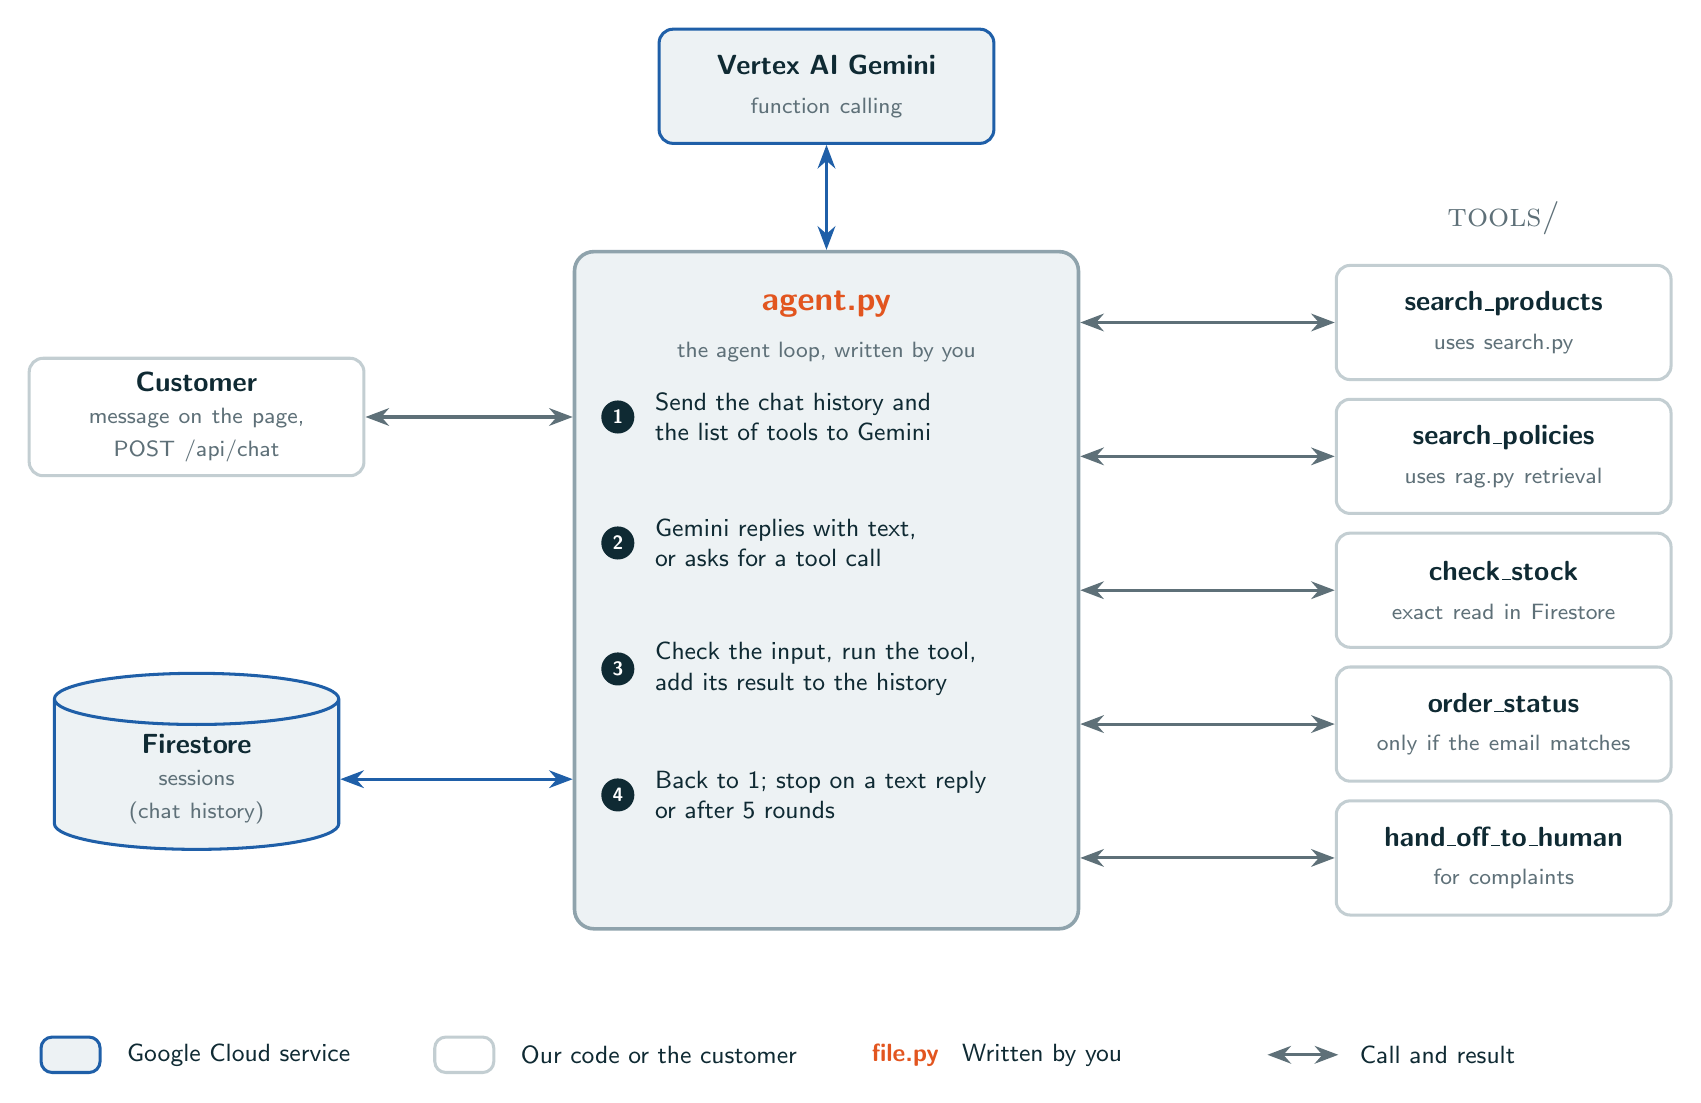
\begin{tikzpicture}[
  font=\sffamily,
  box/.style={rounded corners=5pt, draw=line, line width=1.1pt, fill=white,
    text=ink, align=center, text width=3.9cm, minimum height=1.45cm,
    inner sep=5pt},
  gcp/.style={box, draw=blue, fill=hubfill},
  store/.style={cylinder, shape border rotate=90, aspect=0.18,
    draw=blue, fill=hubfill, line width=1.1pt, text=ink, align=center,
    text width=3.4cm, minimum height=1.9cm, inner sep=3pt},
  one/.style={line width=1.1pt, draw=muted, -{Stealth[length=3mm]}},
  two/.style={line width=1.1pt, draw=muted,
    {Stealth[length=3mm]}-{Stealth[length=3mm]}},
  btwo/.style={two, draw=blue},
  loopstep/.style={text=ink, font=\small, align=left, anchor=west},
  num/.style={circle, fill=ink, text=white, font=\scriptsize\bfseries,
    inner sep=1.2pt, minimum size=0.42cm},
]

% ---- The agent loop (hub) ----
\node[rounded corners=7pt, draw=hubline, line width=1.3pt, fill=hubfill,
      minimum width=6.4cm, minimum height=8.6cm] (hub) at (0,0) {};
\node[text=orange, font=\large\bfseries, anchor=north] at ([yshift=-0.4cm]hub.north)
  {agent.py};
\node[text=muted, font=\footnotesize, anchor=north] at ([yshift=-1.05cm]hub.north)
  {the agent loop, written by you};

\node[num] (n1) at (-2.65, 2.2) {1};
\node[loopstep, text width=4.9cm] at (-2.3, 2.2)
  {Send the chat history and\\the list of tools to Gemini};
\node[num] (n2) at (-2.65, 0.6) {2};
\node[loopstep, text width=4.9cm] at (-2.3, 0.6)
  {Gemini replies with text,\\or asks for a tool call};
\node[num] (n3) at (-2.65,-1.0) {3};
\node[loopstep, text width=4.9cm] at (-2.3,-1.0)
  {Check the input, run the tool,\\add its result to the history};
\node[num] (n4) at (-2.65,-2.6) {4};
\node[loopstep, text width=4.9cm] at (-2.3,-2.6)
  {Back to 1; stop on a text reply\\or after 5 rounds};

% ---- Above: Gemini ----
\node[gcp] (gem) at (0, 6.4)
  {\lbl{Vertex AI Gemini}{function calling}};
\draw[btwo] (gem.south) -- (hub.north);

% ---- Left: customer and session ----
\node[box] (cust) at (-8.0, 2.2)
  {\lbl{Customer}{message on the page,\\POST /api/chat}};
\node[store] (sess) at (-8.0,-2.4)
  {\lbl{Firestore}{sessions\\(chat history)}};
\draw[two] (cust.east) -- (cust.east -| hub.west);
\draw[btwo] (sess.east) -- (sess.east -| hub.west);

% ---- Right: the tools ----
\def\tx{8.6}
\node[box] (t1) at (\tx, 3.4)  {\lbl{search\_products}{uses search.py}};
\node[box] (t2) at (\tx, 1.7)  {\lbl{search\_policies}{uses rag.py retrieval}};
\node[box] (t3) at (\tx, 0.0)  {\lbl{check\_stock}{exact read in Firestore}};
\node[box] (t4) at (\tx,-1.7)  {\lbl{order\_status}{only if the email matches}};
\node[box] (t5) at (\tx,-3.4)  {\lbl{hand\_off\_to\_human}{for complaints}};
\foreach \t in {t1,t2,t3,t4,t5}
  \draw[two] (\t.west -| hub.east) -- (\t.west);
\node[text=muted, font=\large\scshape, anchor=south] at ([yshift=0.25cm]t1.north)
  {tools/};

% ---- Legend ----
\node[rounded corners=4pt, draw=blue, line width=1.1pt, fill=hubfill,
      minimum width=0.75cm, minimum height=0.45cm] (k1) at (-9.6,-5.9) {};
\node[anchor=west, text=ink, font=\small] at ([xshift=0.2cm]k1.east)
  {Google Cloud service};
\node[rounded corners=4pt, draw=line, line width=1.1pt, fill=white,
      minimum width=0.75cm, minimum height=0.45cm] (k2) at (-4.6,-5.9) {};
\node[anchor=west, text=ink, font=\small] at ([xshift=0.2cm]k2.east)
  {Our code or the customer};
\node[text=orange, font=\small\bfseries] (k3) at (1.0,-5.9) {file.py};
\node[anchor=west, text=ink, font=\small] at ([xshift=0.05cm]k3.east)
  {Written by you};
\draw[two] (5.6,-5.9) -- (6.5,-5.9);
\node[anchor=west, text=ink, font=\small] at (6.65,-5.9) {Call and result};

\end{tikzpicture}
\end{document}
